\documentclass[12pt]{report} % You can use 'article' or 'book' class as well

\usepackage{graphicx} % For including images
\usepackage{minted}

\begin{document}

% Title page
\begin{titlepage}
	\centering
	\vspace*{1cm} % Adjusts vertical space for the image
	% Insert your image (use the actual path and filename of your image)
	
\includegraphics[width=0.3\textwidth]{../../images/KMITL Logo.png} % Adjust width as needed

	\vspace{1cm} % Vertical space after the image
	{\LARGE \textbf{Homework 6}} \\[0.5cm] % Title
	\vspace{0.5cm}
	{\large \textbf{01286233 Web Programming}} \\[0.5cm]
	{\large \textbf{Software Engineering Program,}} \\[0.5cm]
	{\large \textbf{Department of Computer Engineering,}} \\[0.5cm]
	{\large \textbf{School of Engineering, KMITL}} \\[1cm]
	{\Large 67011352 Theepakorn Phayonrat} \\[0.5cm] % Authors (Use \\ the separate authors)
\end{titlepage}

\section*{Code}

\subsection*{HW6\_67011352\_Theepakorn.html}

\begin{minted}[fontsize=\small, breaklines, breakanywhere, breakindent=1em]{html}
<!DOCTYPE html>
<html lang="en">
    <head>
        <meta charset="UTF-8">
        <meta name="viewport" content="width=device-width, initial-scale=1">
        <title>Calendar</title>
        <link href="HW6_67011352_Theepakorn.css" rel="stylesheet">
    </head>
    <body>
        <div class="container">
            <table id="calendar">
                <thead>
                    <tr class="header">
                        <th style="background-color: green;" id="previous"> < </th>
                        <th colspan="5" id="monthHeader">Loading...</th>
                        <th style="background-color: green;" id="next"> > </th>
                    </tr>
                </thead>
                <tbody>
                    <tr class="header">
                        <td>Mon</td>
                        <td>Tue</td>
                        <td>Wed</td>
                        <td>Thu</td>
                        <td>Fri</td>
                        <td>Sat</td>
                        <td>Sun</td>
                    </tr>
                    <tr id="week1"></tr>
                    <tr id="week2"></tr>
                    <tr id="week3"></tr>
                    <tr id="week4"></tr>
                    <tr id="week5"></tr>
                    <tr id="week6"></tr>
                </tbody>
            </table>
        </div>
        <script src="HW6_67011352_Theepakorn.js"></script>
    </body>
</html>
\end{minted}

\newpage

\subsection*{HW6\_67011352\_Theepakorn.css}

\begin{minted}[fontsize=\small, breaklines, breakanywhere, breakindent=1em]{css}
body {
    margin: 0 auto;
}

.container {
    width: 100%;
    height: 100vh;
    display: flex;
    margin: 0 auto;
    align-items: center;
    justify-content: center;
}

table {
    border: solid 1px black;
    border-collapse: collapse;
}

.header {
    height: 25px;
}

th, td {
    width: 50px;
    height: 50px;
    text-align: center;
    border: 1px solid black;
}
\end{minted}

\newpage

\subsection*{HW6\_67011352\_Theepakorn.js}

\begin{minted}[fontsize=\small, breakindent=1em]{js}
// Every function here use the quirk of Javascript Array that it
// passes into function by its reference. Therefore, we can keep track
// of the value inside the currentData Array.
const MAX_DATE = [31, 28, 31, 30, 31, 30, 31, 31 ,30, 31, 30, 31];
const calendar = document.getElementById("calendar");
const previousButton = document.getElementById("previous");
const nextButton = document.getElementById("next");
let currentData = [8, 5]; // [currentMonth, currentStartIndex]
// The current month is set to August when being loaded

// Render month depending from the currentData
function renderMonth(data, maxDate) {
    // Monday of the 1st week is startIndex = 1 and the start of
    // August is startIndex = 5 AKA 1st week Friday
    const month = data[0];
    const startIndex = data[1];

    const currentMaxDate = maxDate[month - 1];
    // currentMonth - 1 because we are random accessing via index
    const weeksNeeded = Math.ceil((currentMaxDate + startIndex - 1)/7);
    // Round up the decimal points to  get the whole new line of week

    const monthHeader = document.getElementById("monthHeader");
    const monthHeaderText = `${month}/2025`; // Like f-String in Python
    monthHeader.innerText = monthHeaderText;

    if (month == 1) { // Cannot go beyond the 12 months boundaries
        previousButton.style = "background-color: red;";
    }
    if (month == 12) {
        nextButton.style = "background-color: red;";
    }

    var date_count = 1;
    var count = 1;

    for (var w = 1; w <= weeksNeeded; w++) {
        const weekString = `week${w}`; // Create a text so that we can
                                       // getElementById the weeks
        const currentWeek = document.getElementById(weekString);
        for (var d = 1; d <= 7; d++) {
            let displayDate = " ";
            if (count >= startIndex && date_count <= currentMaxDate) {
                displayDate = date_count;
                date_count++;
            }
            const currentDay = document.createElement("td");
            currentDay.innerText = displayDate;
            currentWeek.appendChild(currentDay);
            count++;
        }
    }
}

// Render previous month when previousButton is onclick
function previousMonth(data, maxDate) {
    if (data[0] == 1) {
        return;
    }
    clearCalendar(data, maxDate);
    // Calculate the startIndex for previous month
    const previousMaxDate = maxDate[data[0] - 2];
    const currentStartIndex = data[1];
    data[0]--;
    data[1] = (35 - previousMaxDate + currentStartIndex) % 7;
    if (data[1] == 0) {
        data[1] = 7;
    }
    renderMonth(data, maxDate);
}

// Render next month when nextButton is onclick
function nextMonth(data, maxDate) {
    if (data[0] == 12) {
        return;
    }
    clearCalendar(data, maxDate);
    // Calculate the startIndex for next month
    const currentMaxDate = maxDate[data[0] - 1];
    const currentStartIndex = data[1];
    data[0]++;
    data[1] = (currentMaxDate + currentStartIndex) % 7;
    if (data[1] == 0) {
        data[1] = 7;
    }
    renderMonth(data, maxDate);
}

// Clean up before next renderMonth
function clearCalendar(data, maxDate) {
    const month = data[0];
    const startIndex = data[1];

    const currentMaxDate = maxDate[month - 1];
    const weeksNeeded = Math.ceil((currentMaxDate + startIndex - 1)/7);

    // Clear the weekN tr elements ready to be added in the next
    // renderMonth function calls
    for (var w = 1; w <= weeksNeeded; w++) {
        const weekString = `week${w}`;
        const currentWeek = document.getElementById(weekString);
        currentWeek.innerHTML = "";
    }
    // Reset the buttons back to their default color in case of being
    // changed to red
    previousButton.style = "background-color: green;";
    nextButton.style = "background-color: green;";
}

addEventListener("load", () => { renderMonth(currentData, MAX_DATE) }, false);
previousButton.onclick = () => {previousMonth(currentData, MAX_DATE)};
nextButton.onclick = () => {nextMonth(currentData, MAX_DATE)};
\end{minted}

\newpage

\section*{Output}

\subsection*{January}
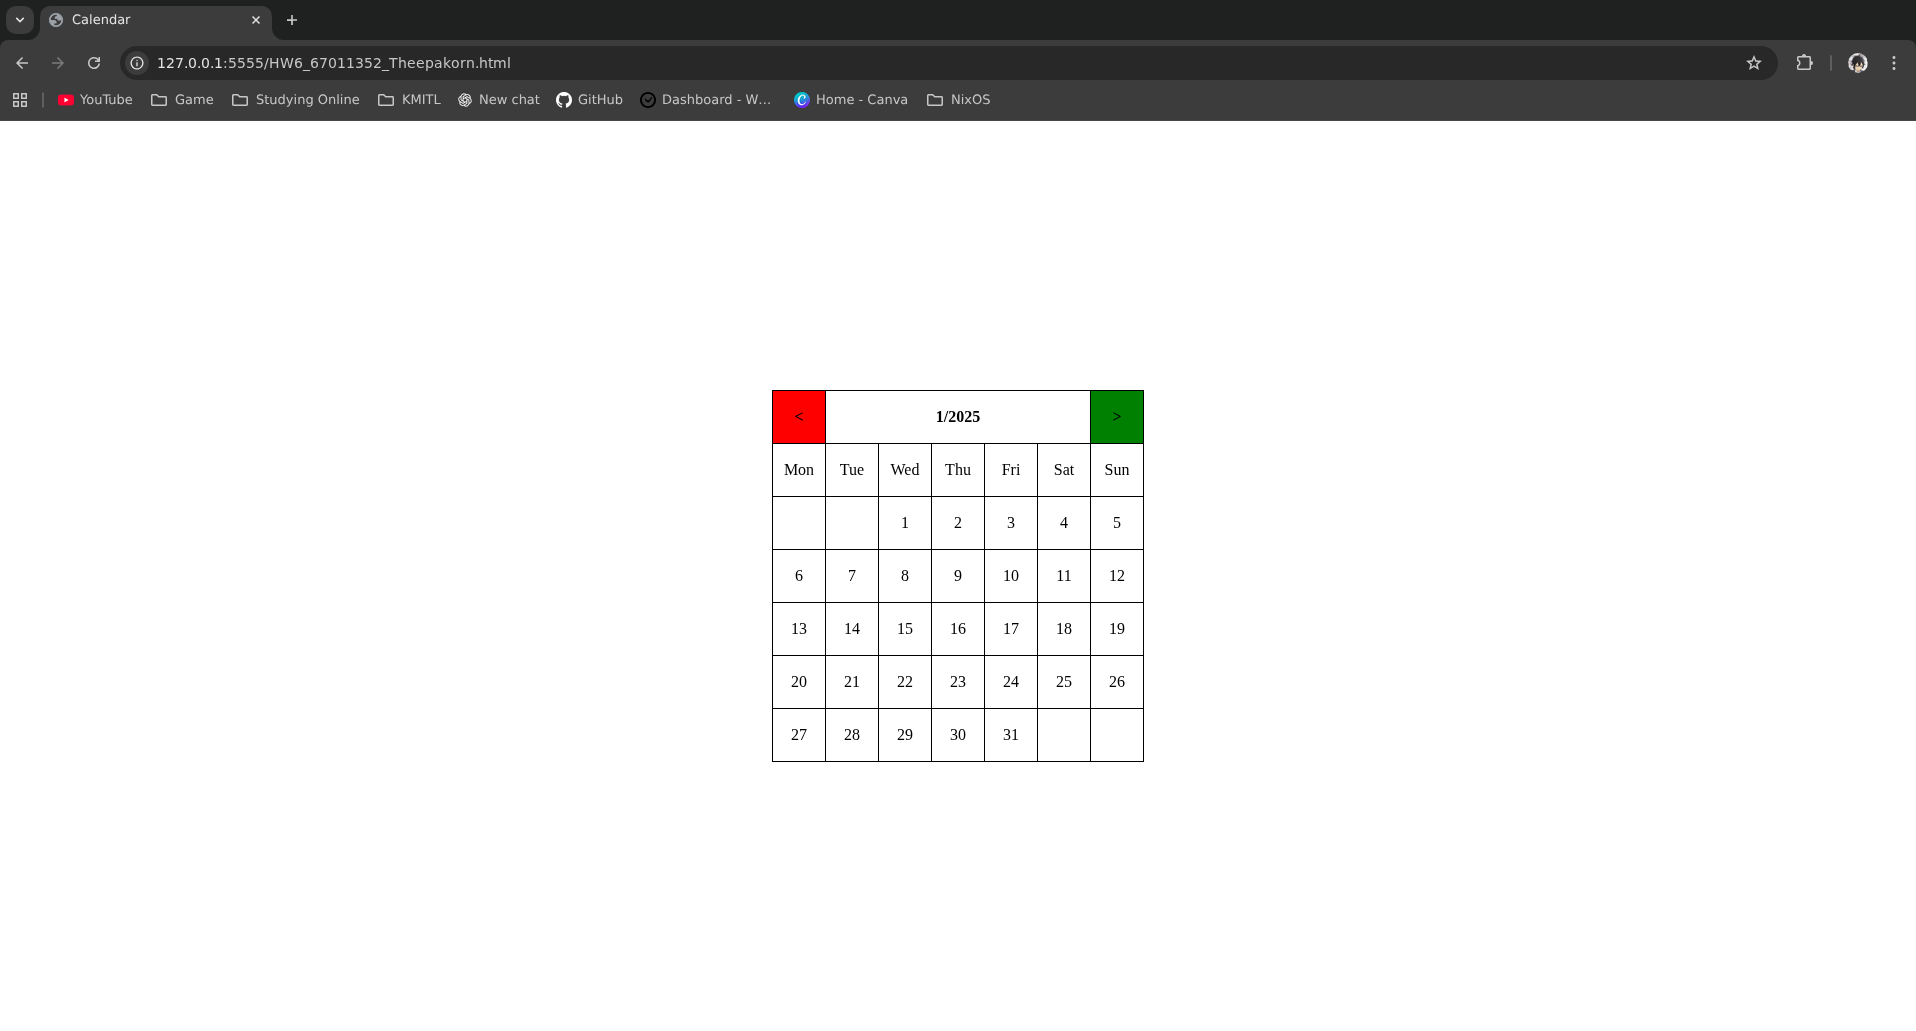
\includegraphics[width=12cm]{./images/Output01.png} \\
\subsection*{February}
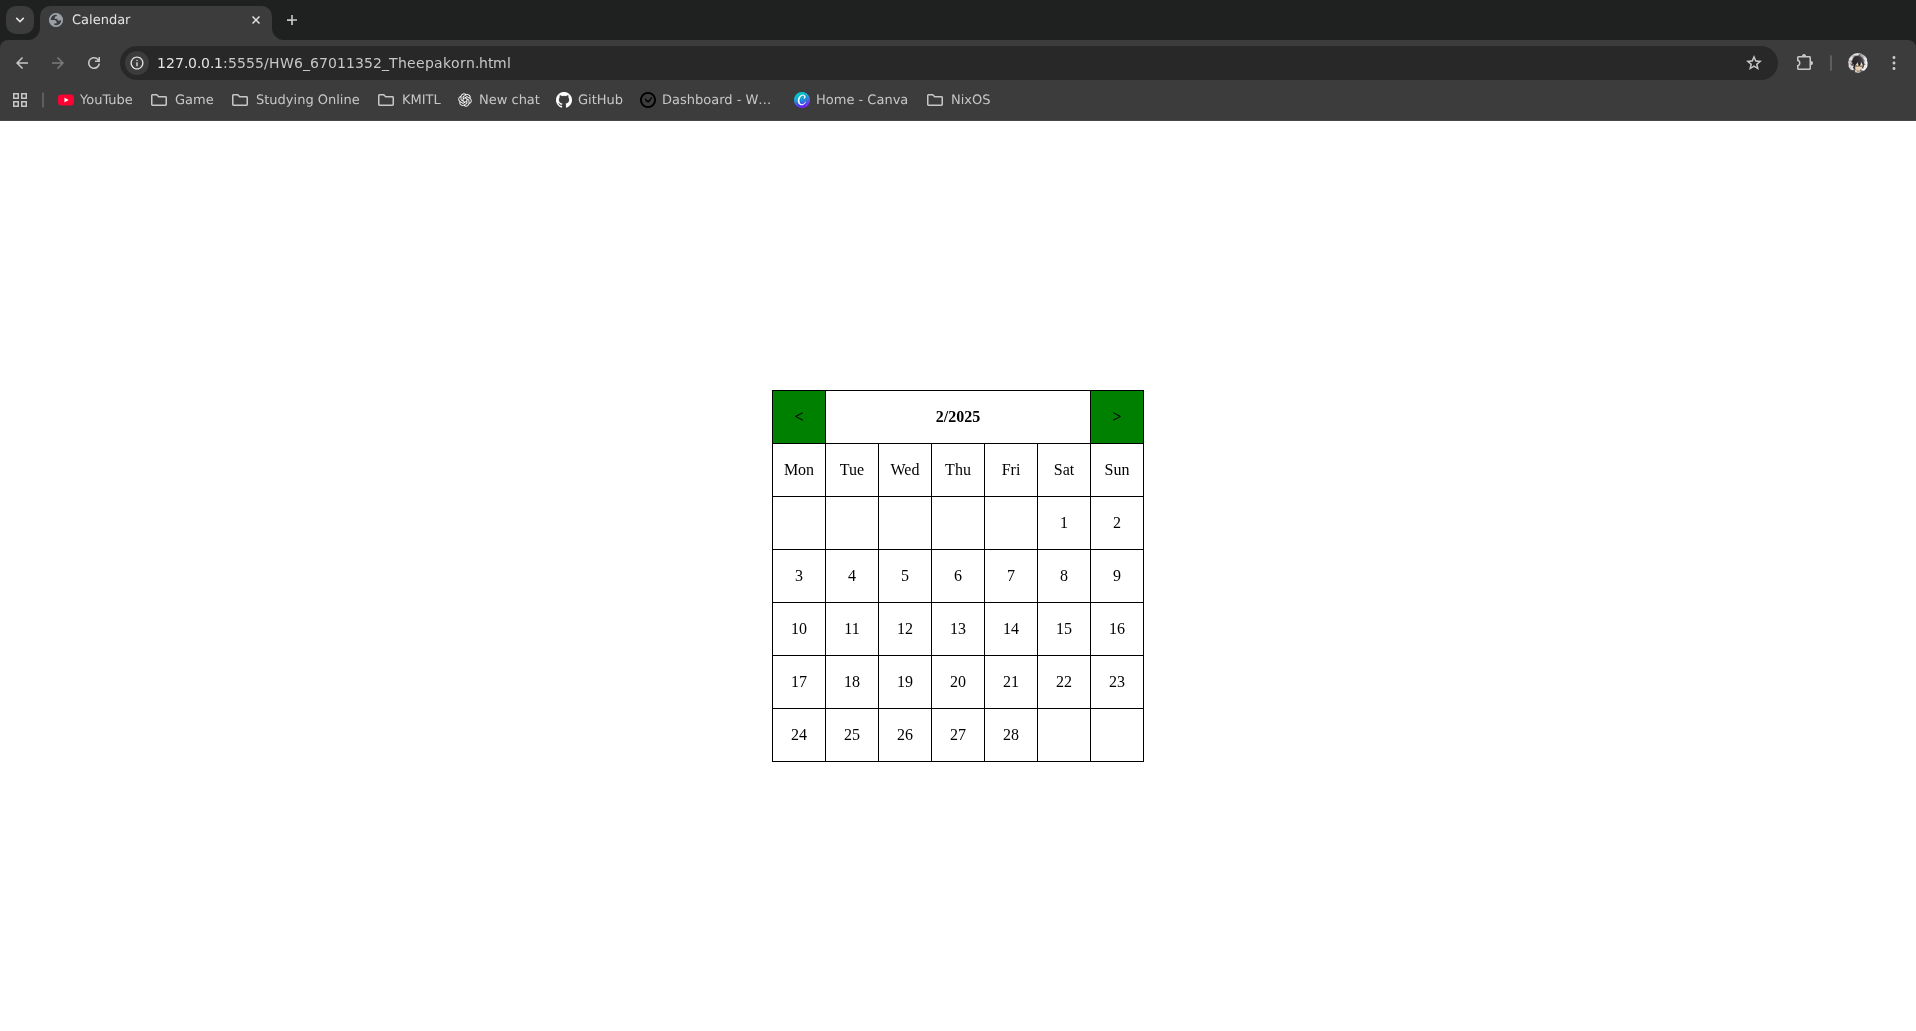
\includegraphics[width=12cm]{./images/Output02.png} \\
\subsection*{March}
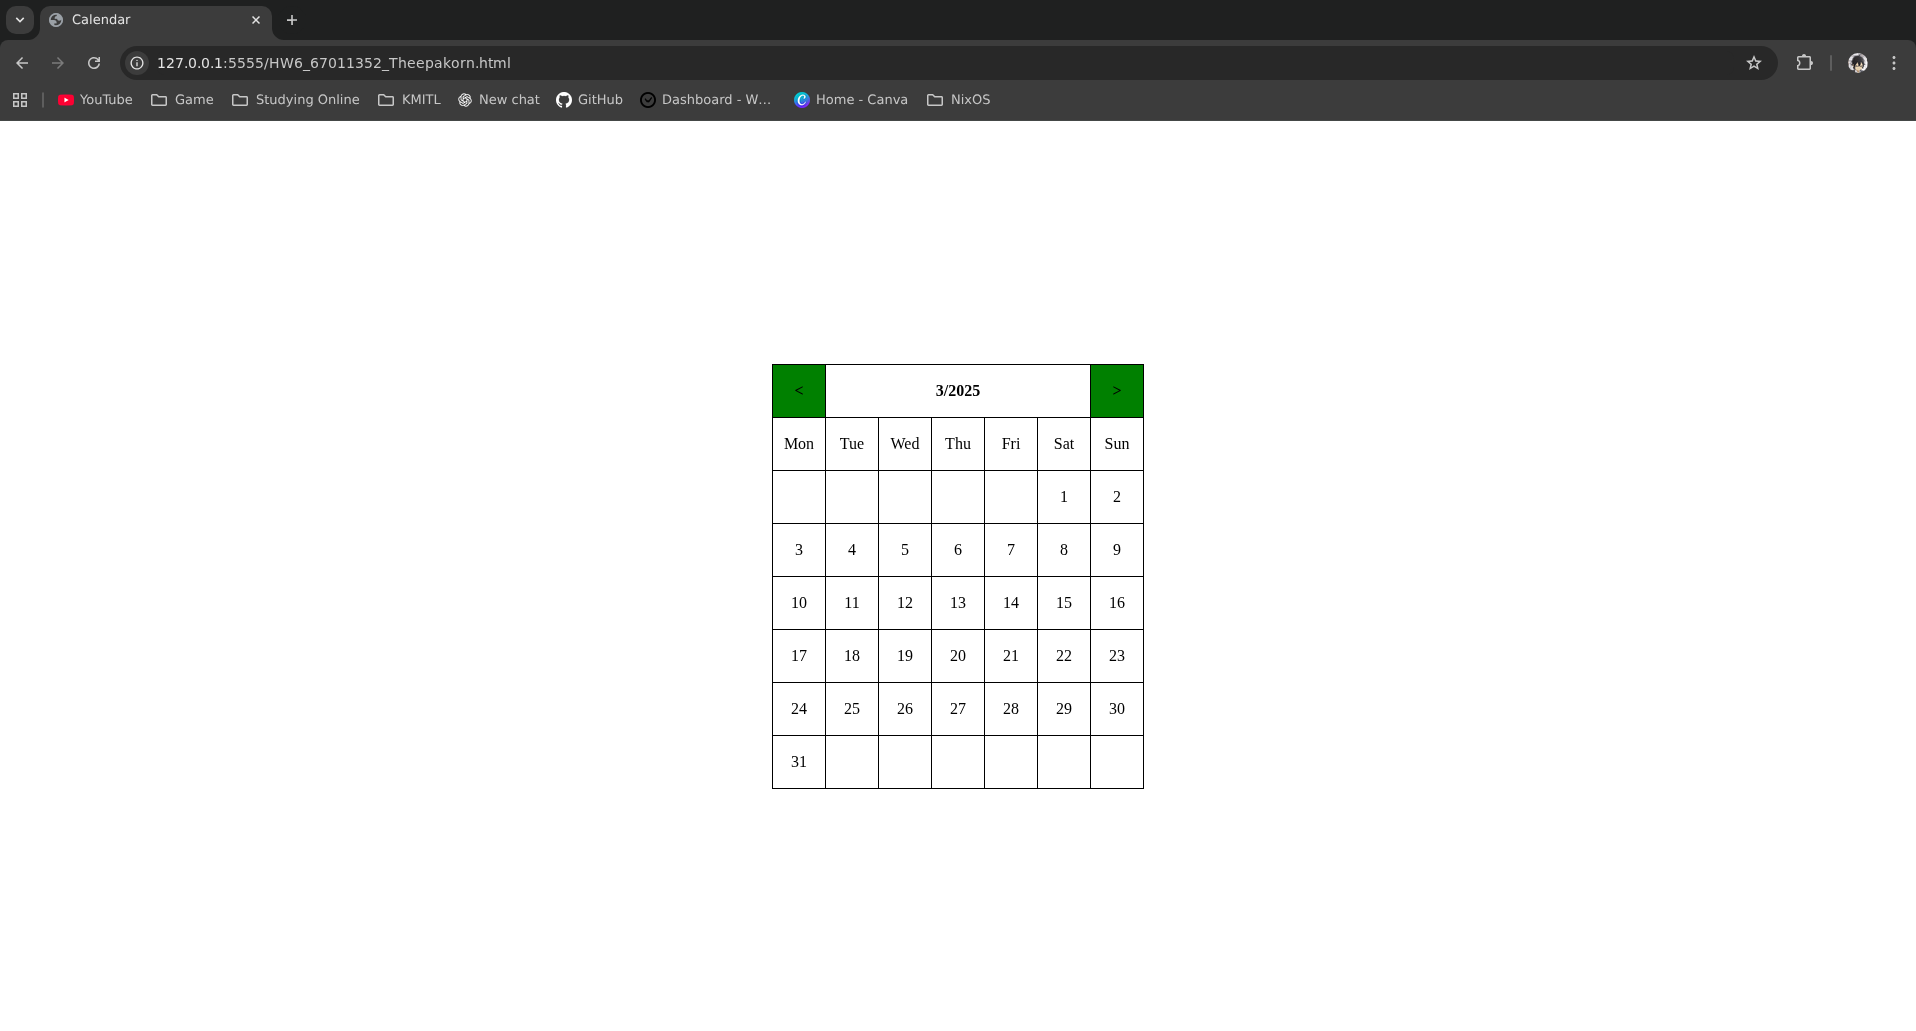
\includegraphics[width=12cm]{./images/Output03.png} \\
\subsection*{April}
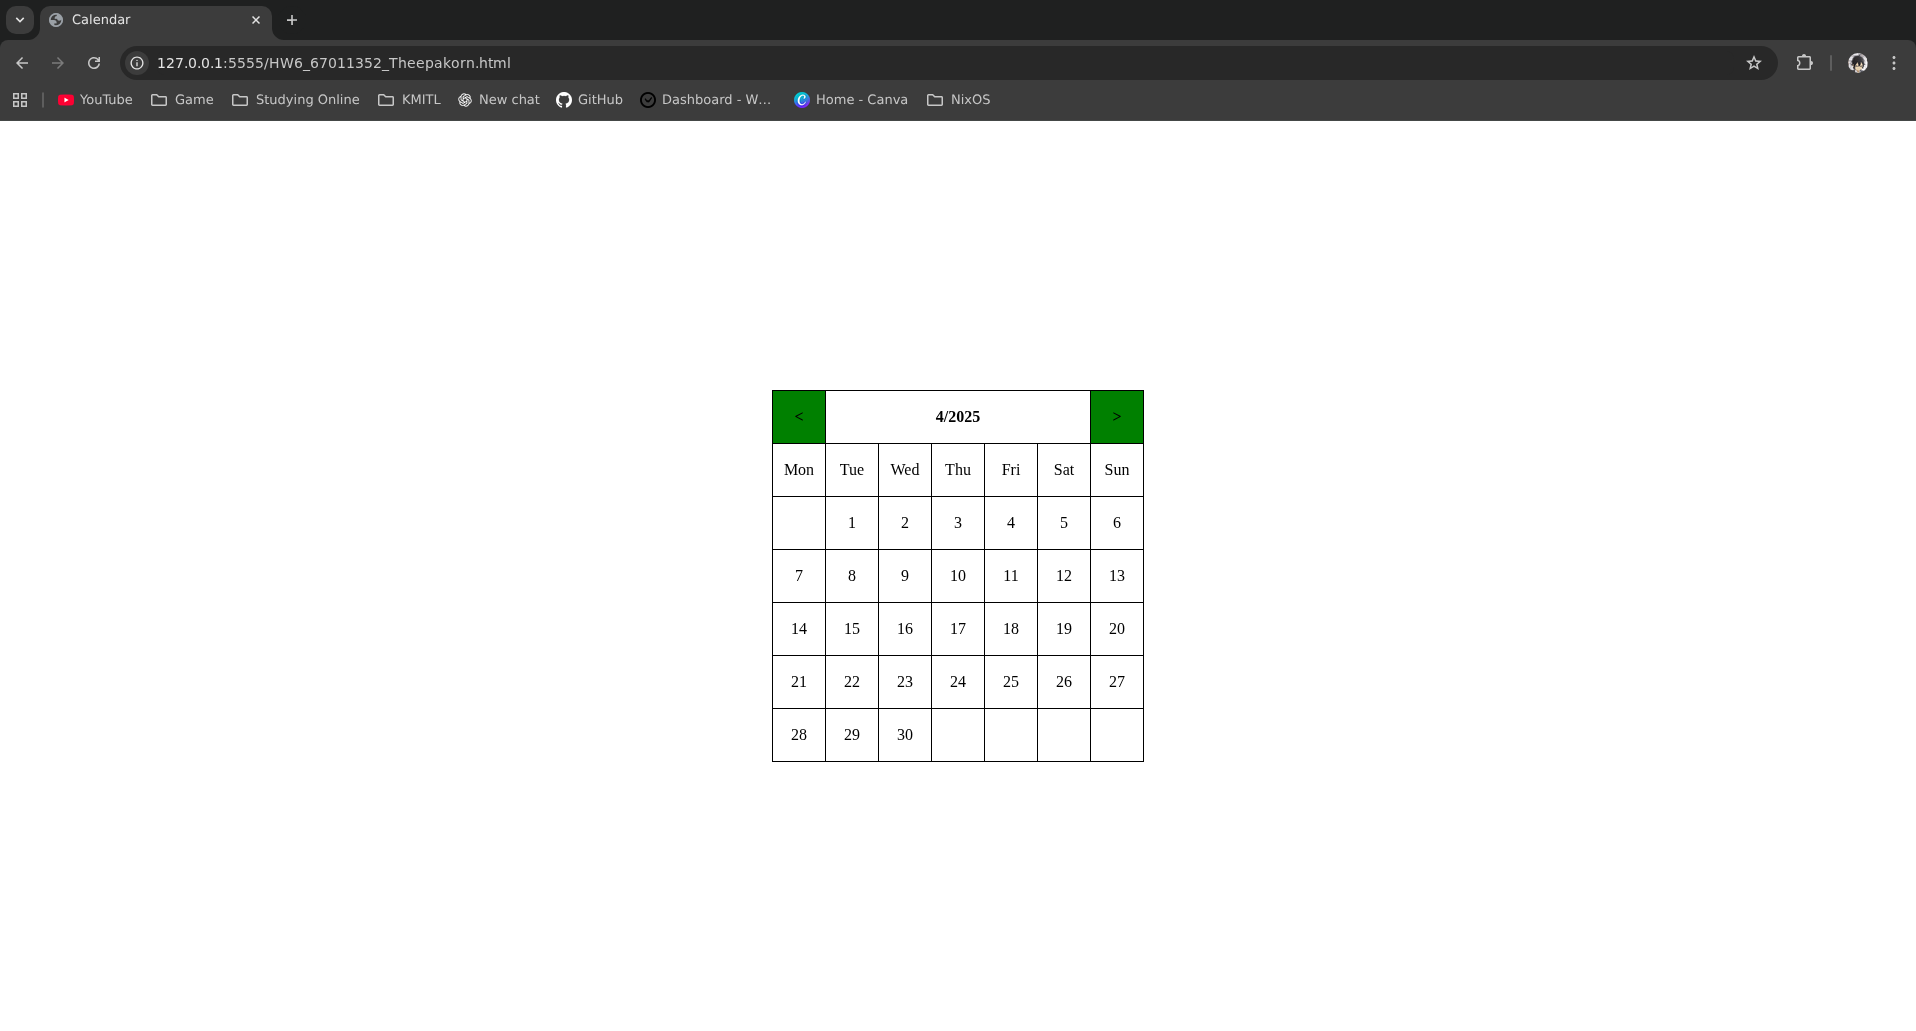
\includegraphics[width=12cm]{./images/Output04.png} \\
\subsection*{May}
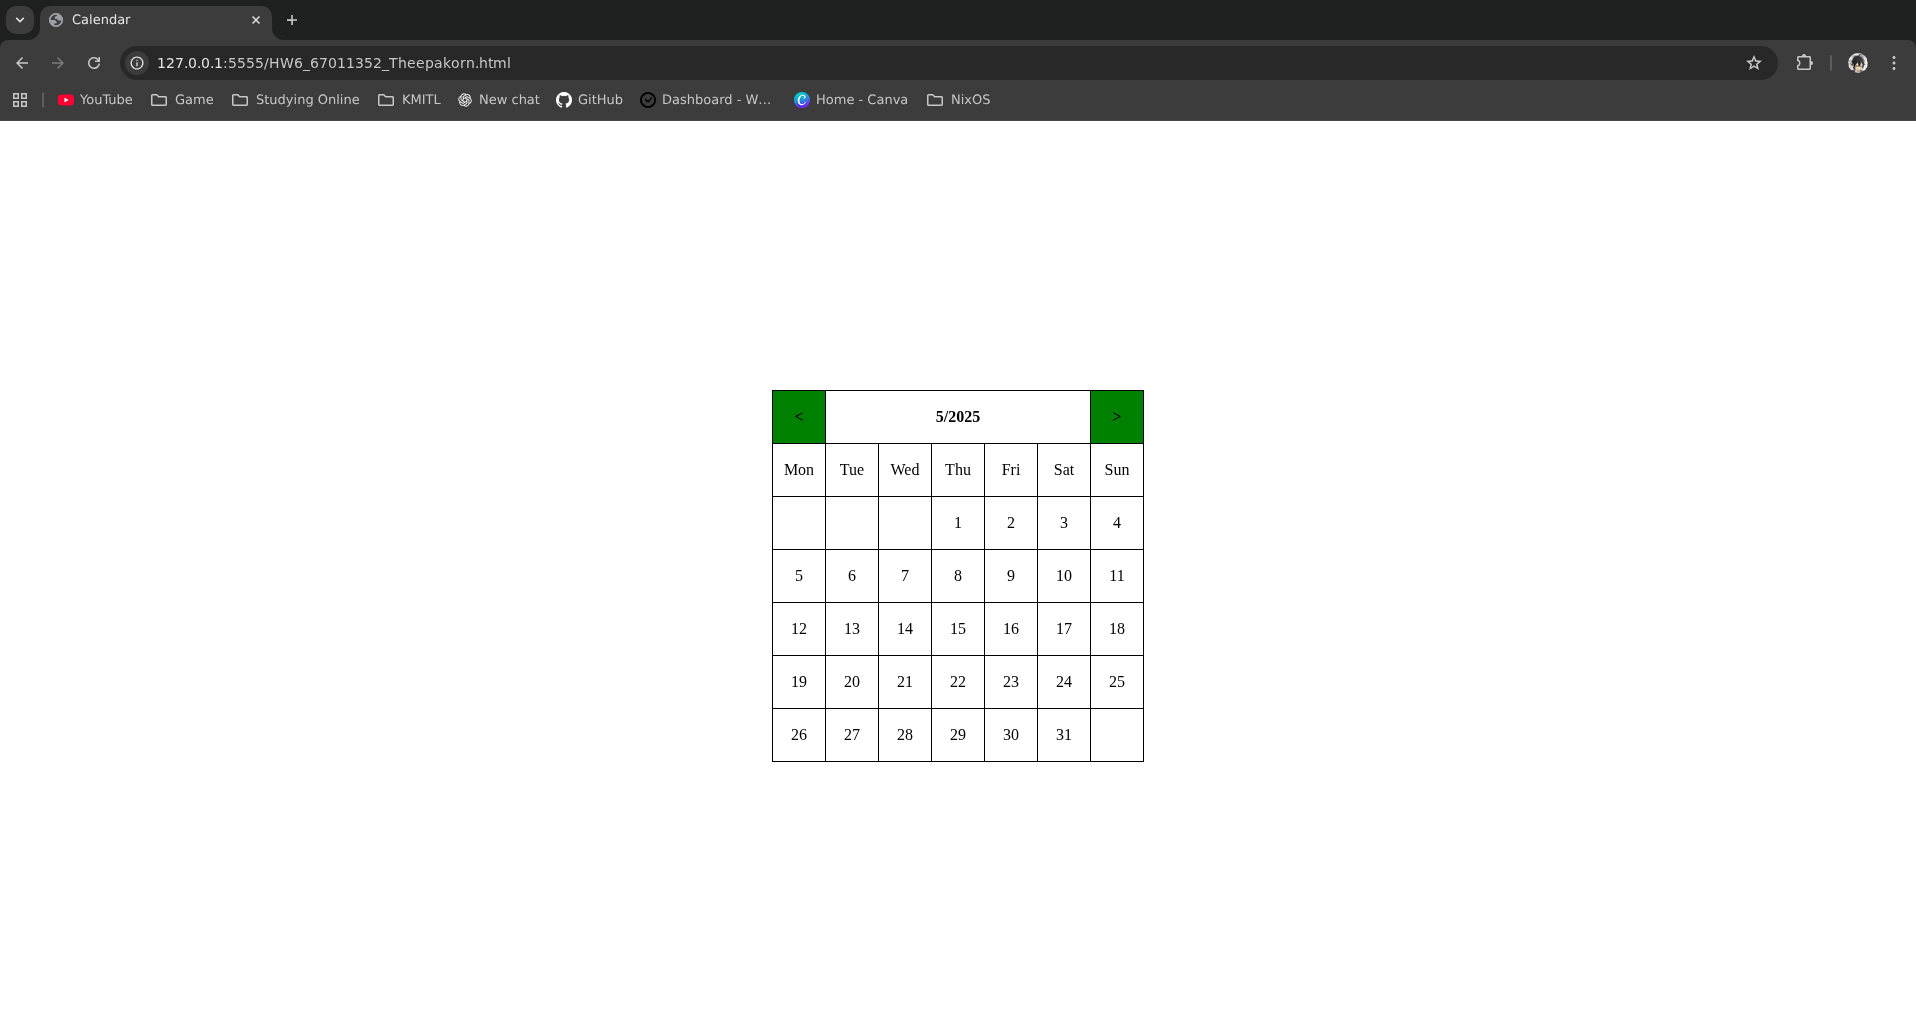
\includegraphics[width=12cm]{./images/Output05.png} \\
\subsection*{June}
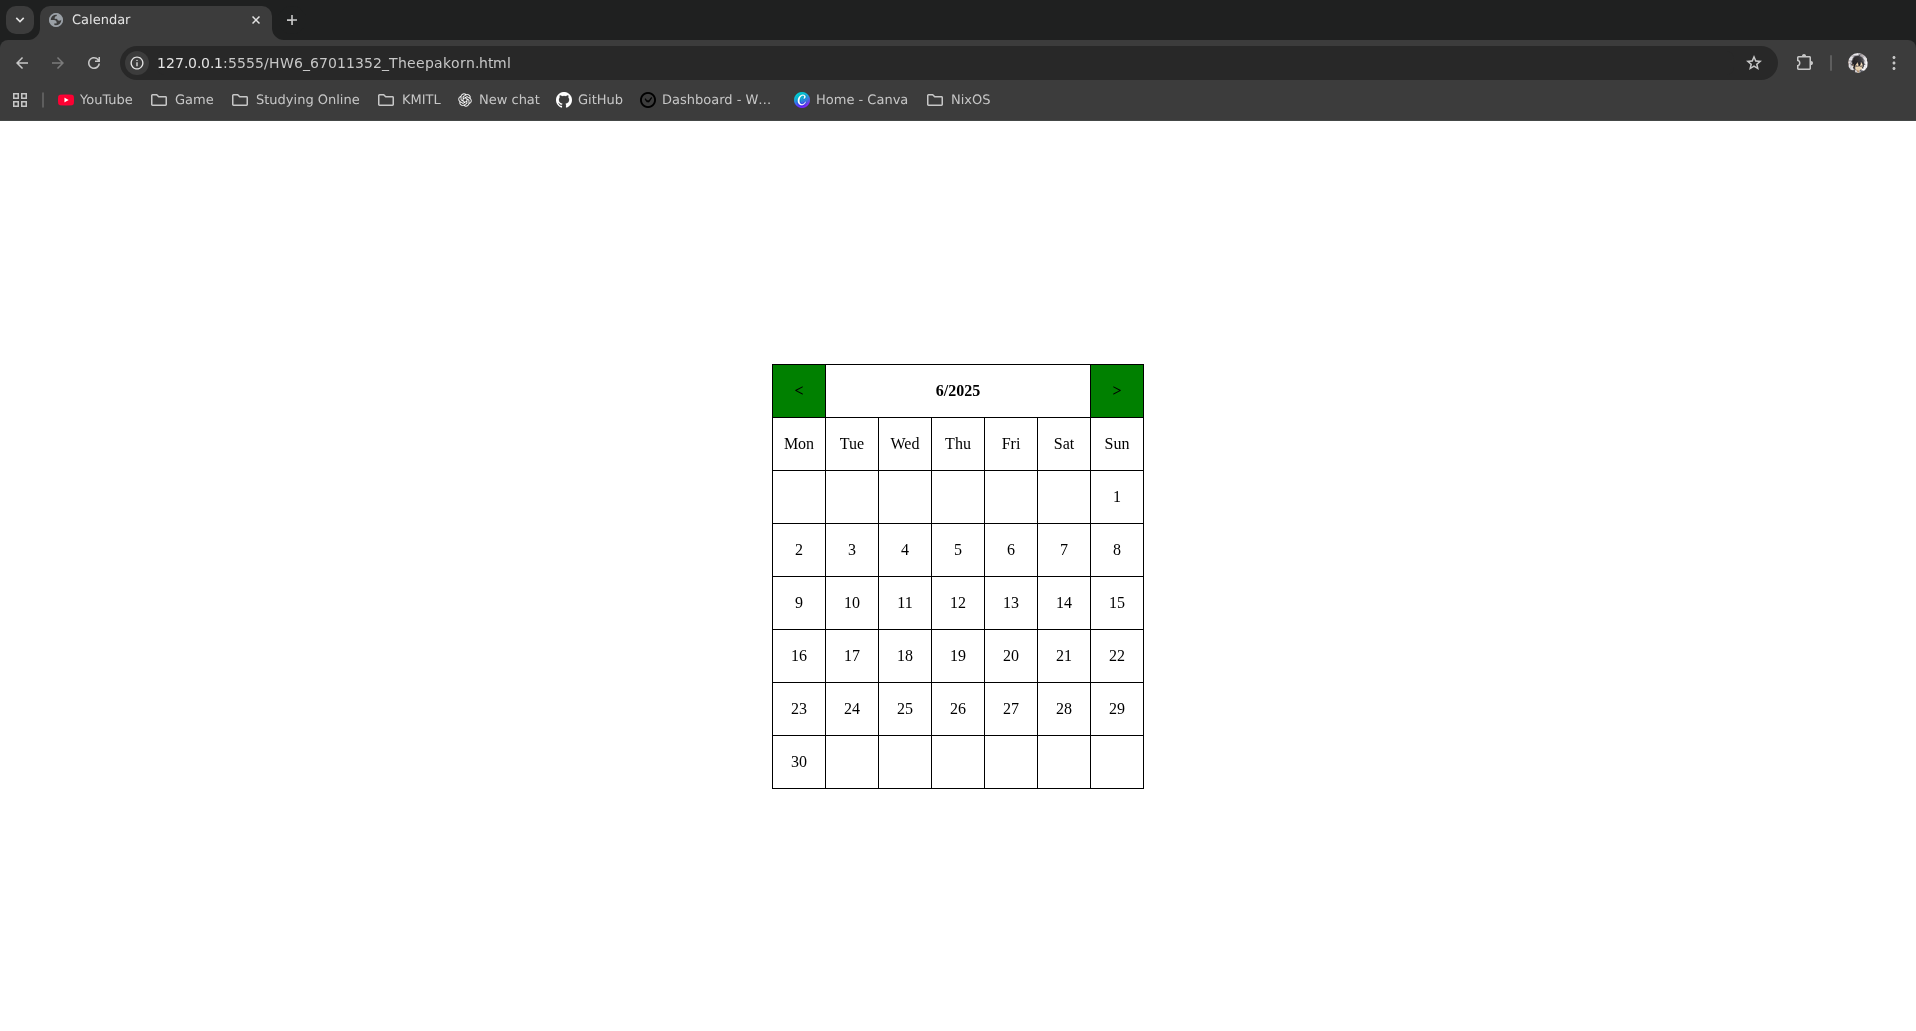
\includegraphics[width=12cm]{./images/Output06.png} \\
\subsection*{July}
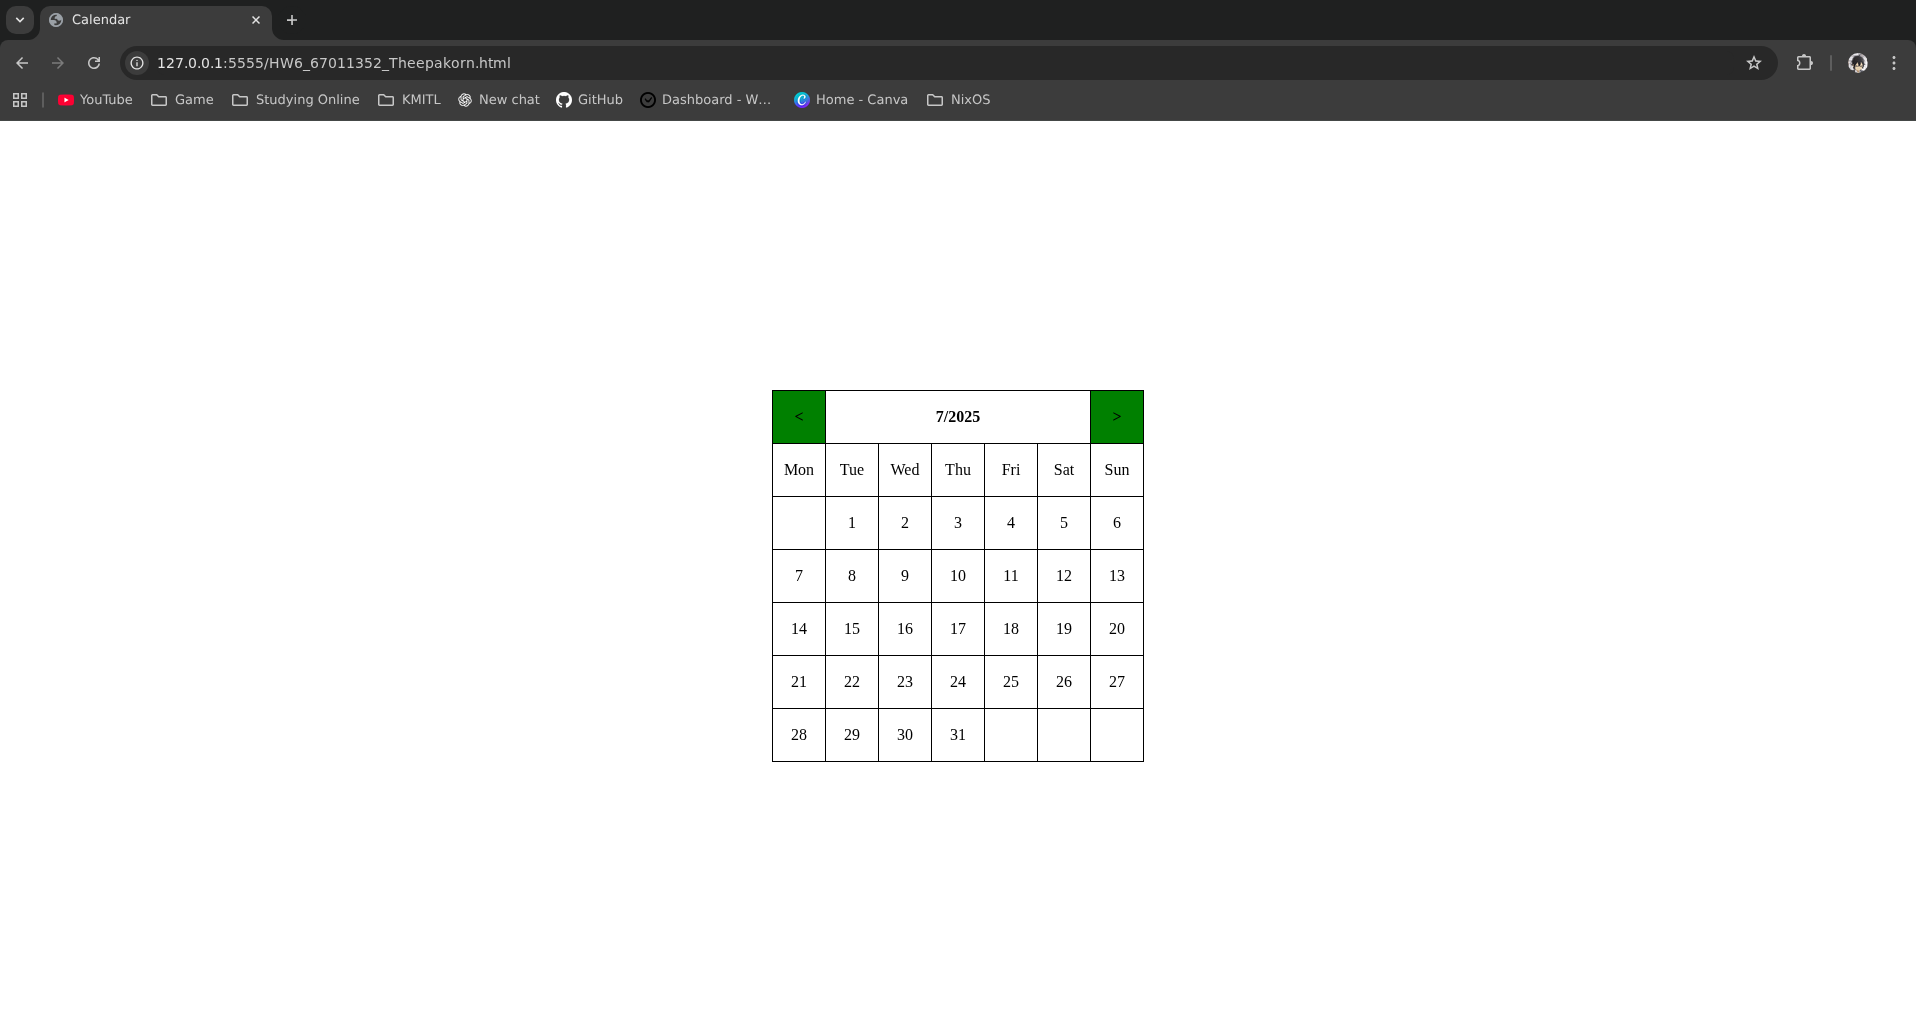
\includegraphics[width=12cm]{./images/Output07.png} \\
\subsection*{August}
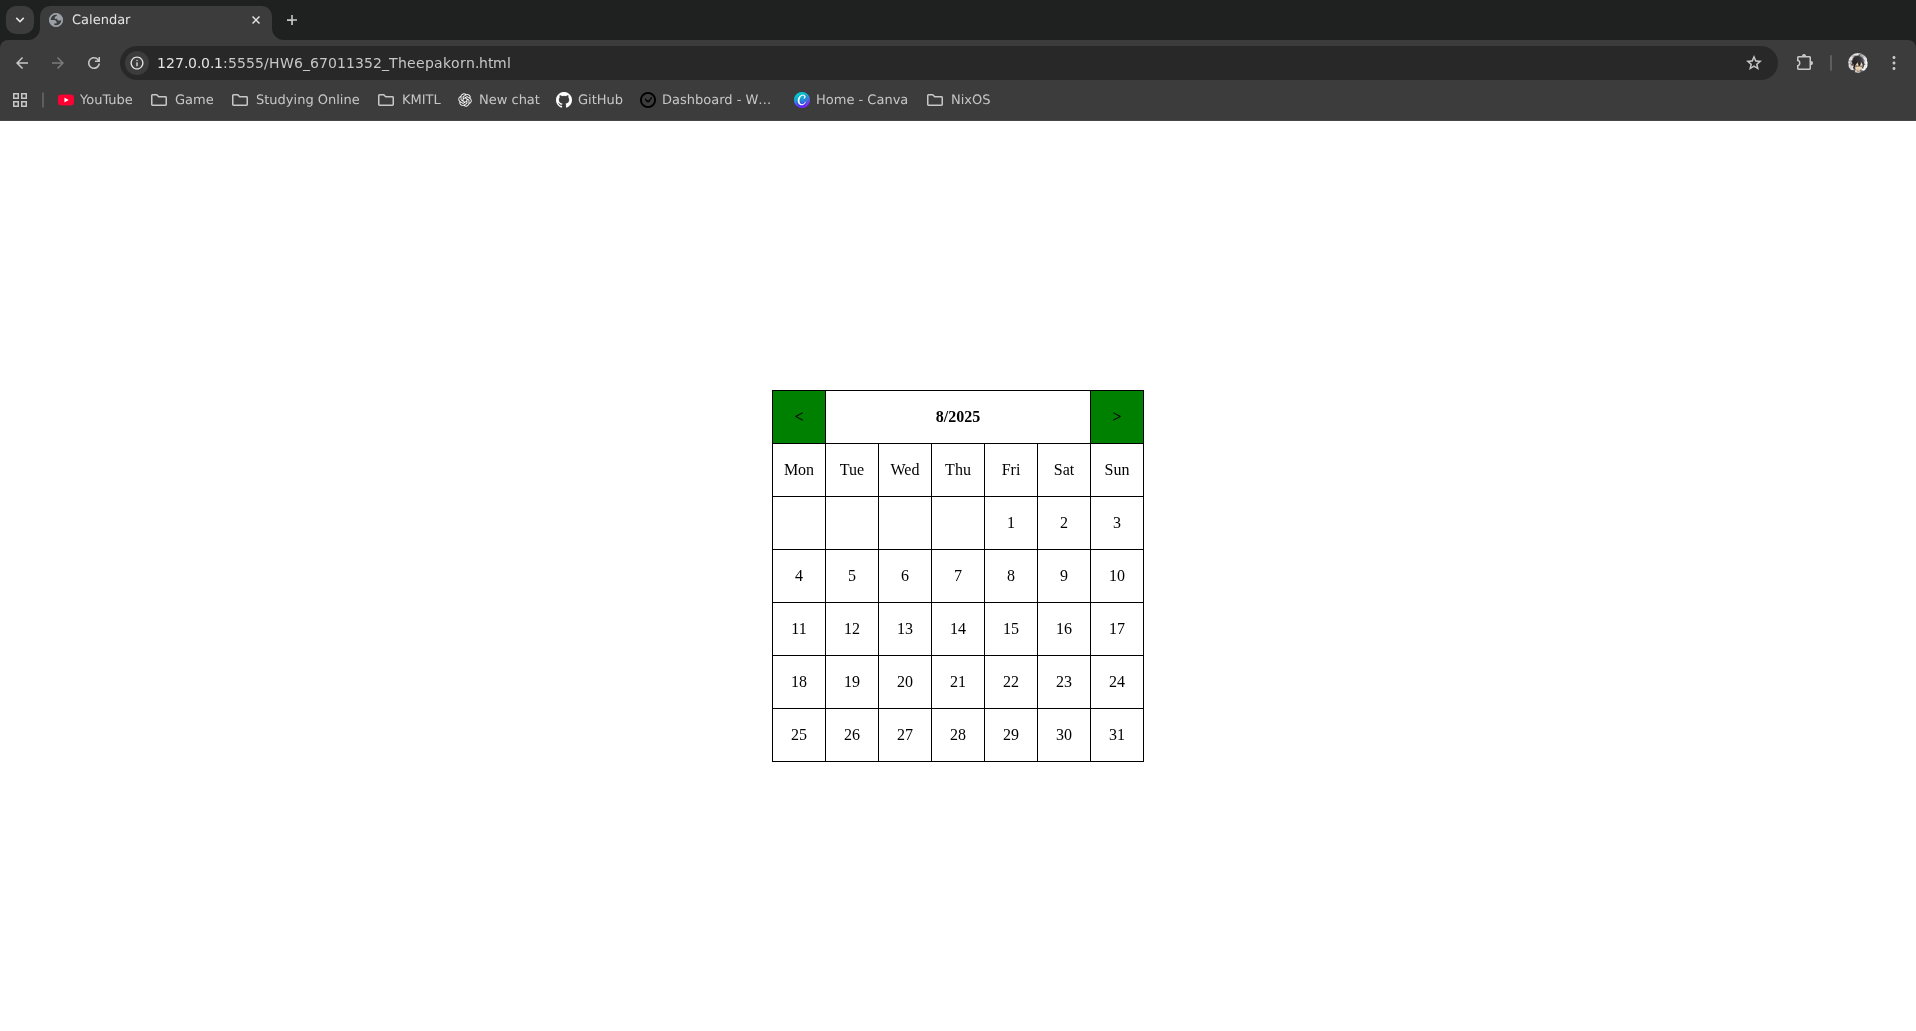
\includegraphics[width=12cm]{./images/Output08.png} \\
\subsection*{September}
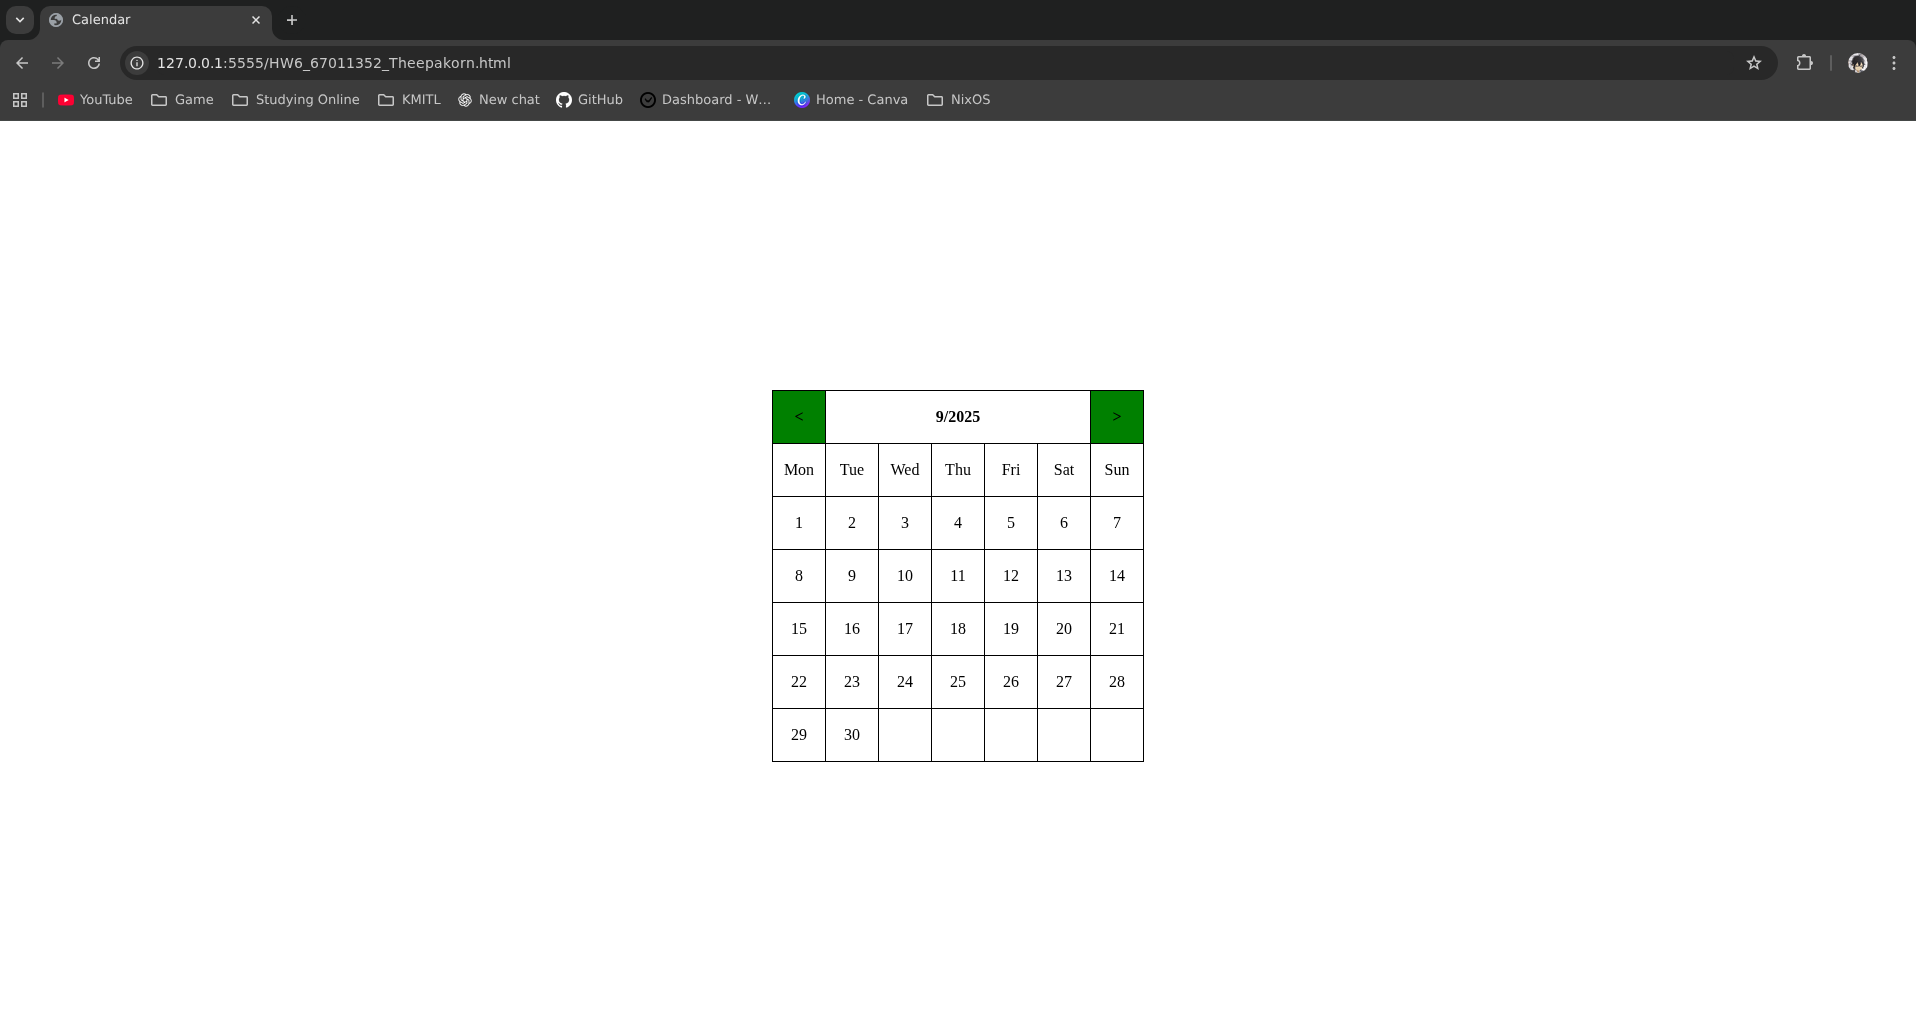
\includegraphics[width=12cm]{./images/Output09.png} \\
\subsection*{October}
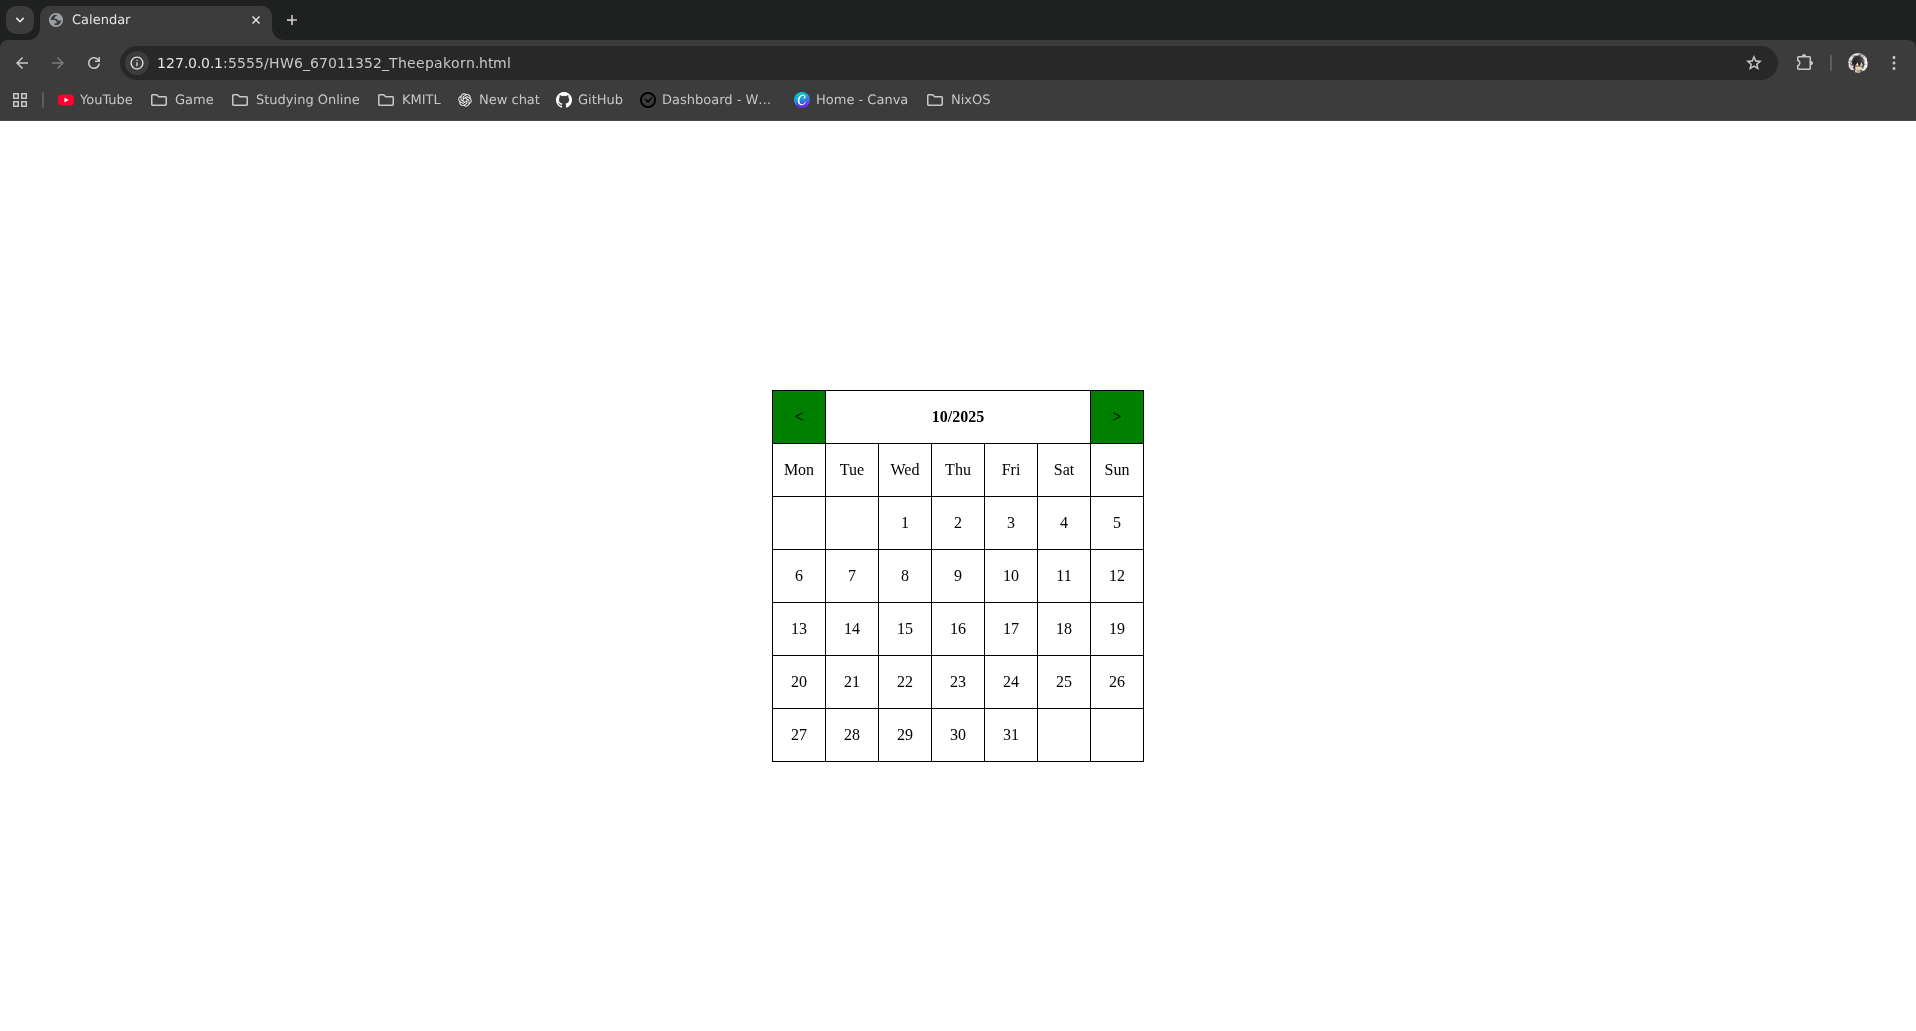
\includegraphics[width=12cm]{./images/Output10.png} \\
\subsection*{November}
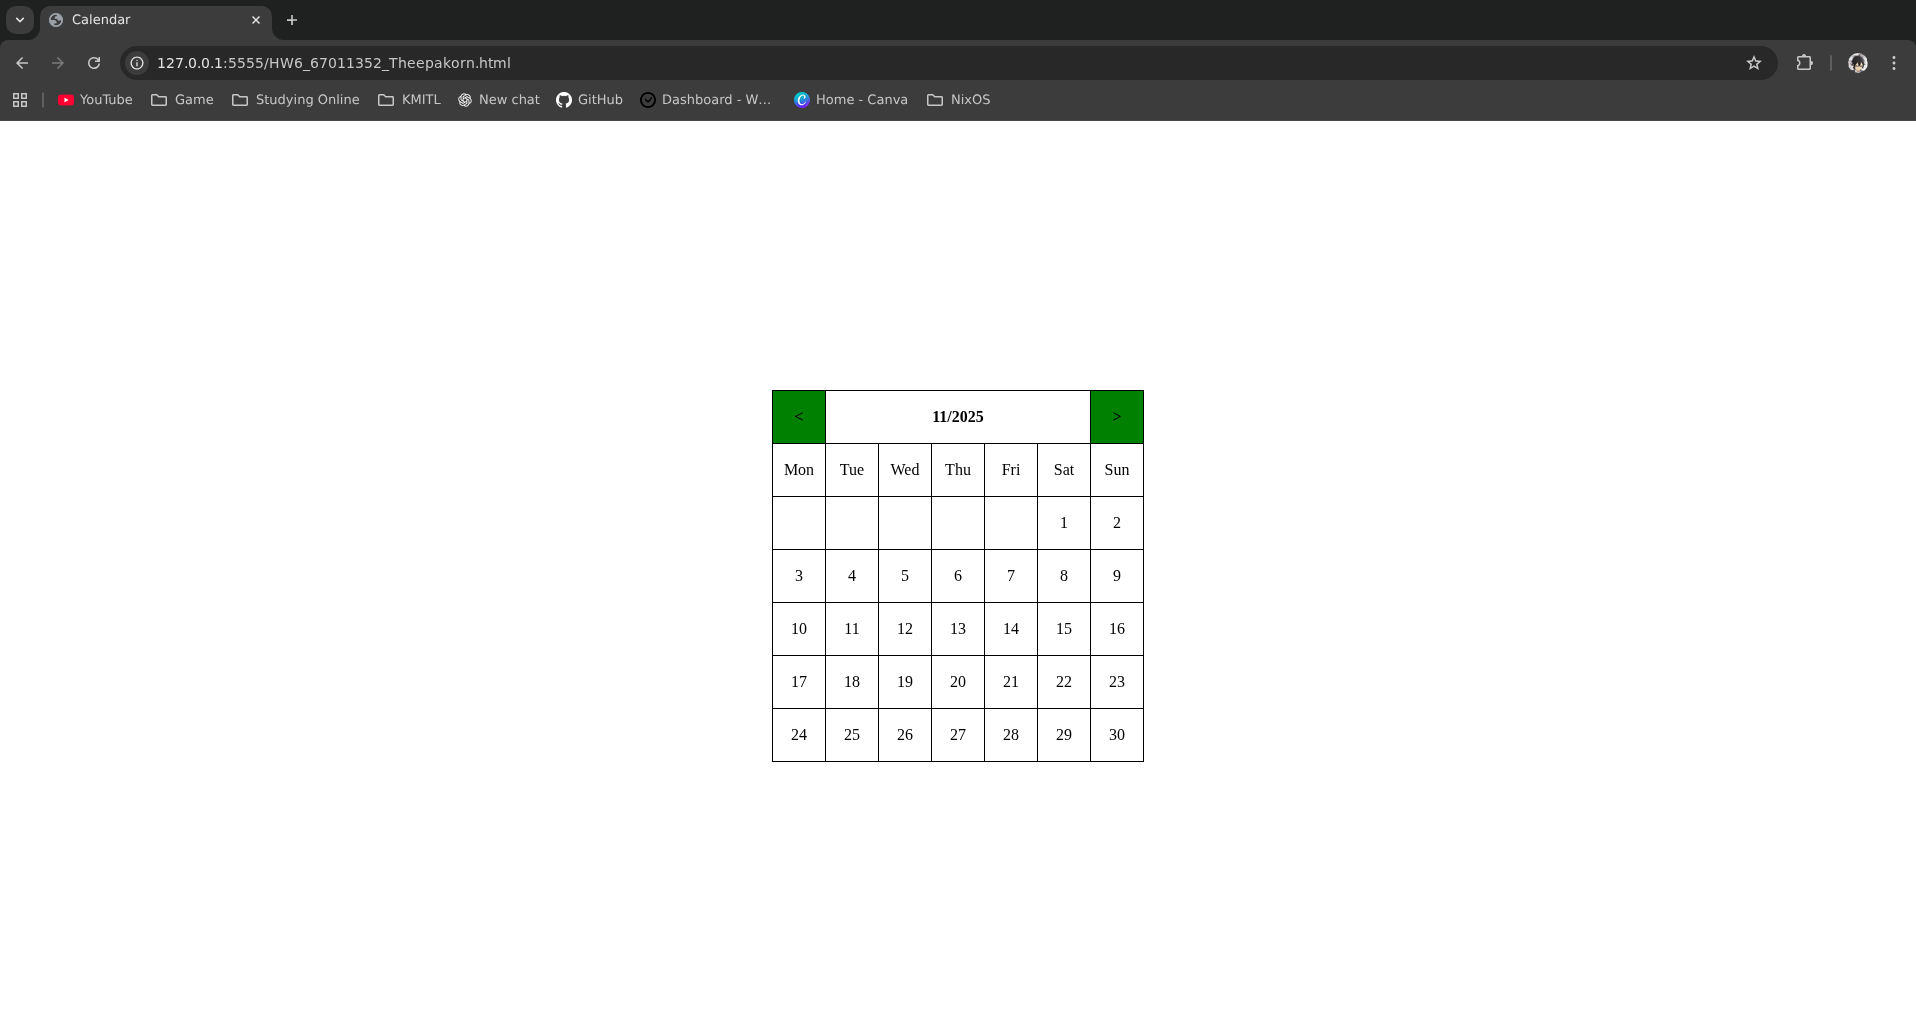
\includegraphics[width=12cm]{./images/Output11.png} \\
\subsection*{December}
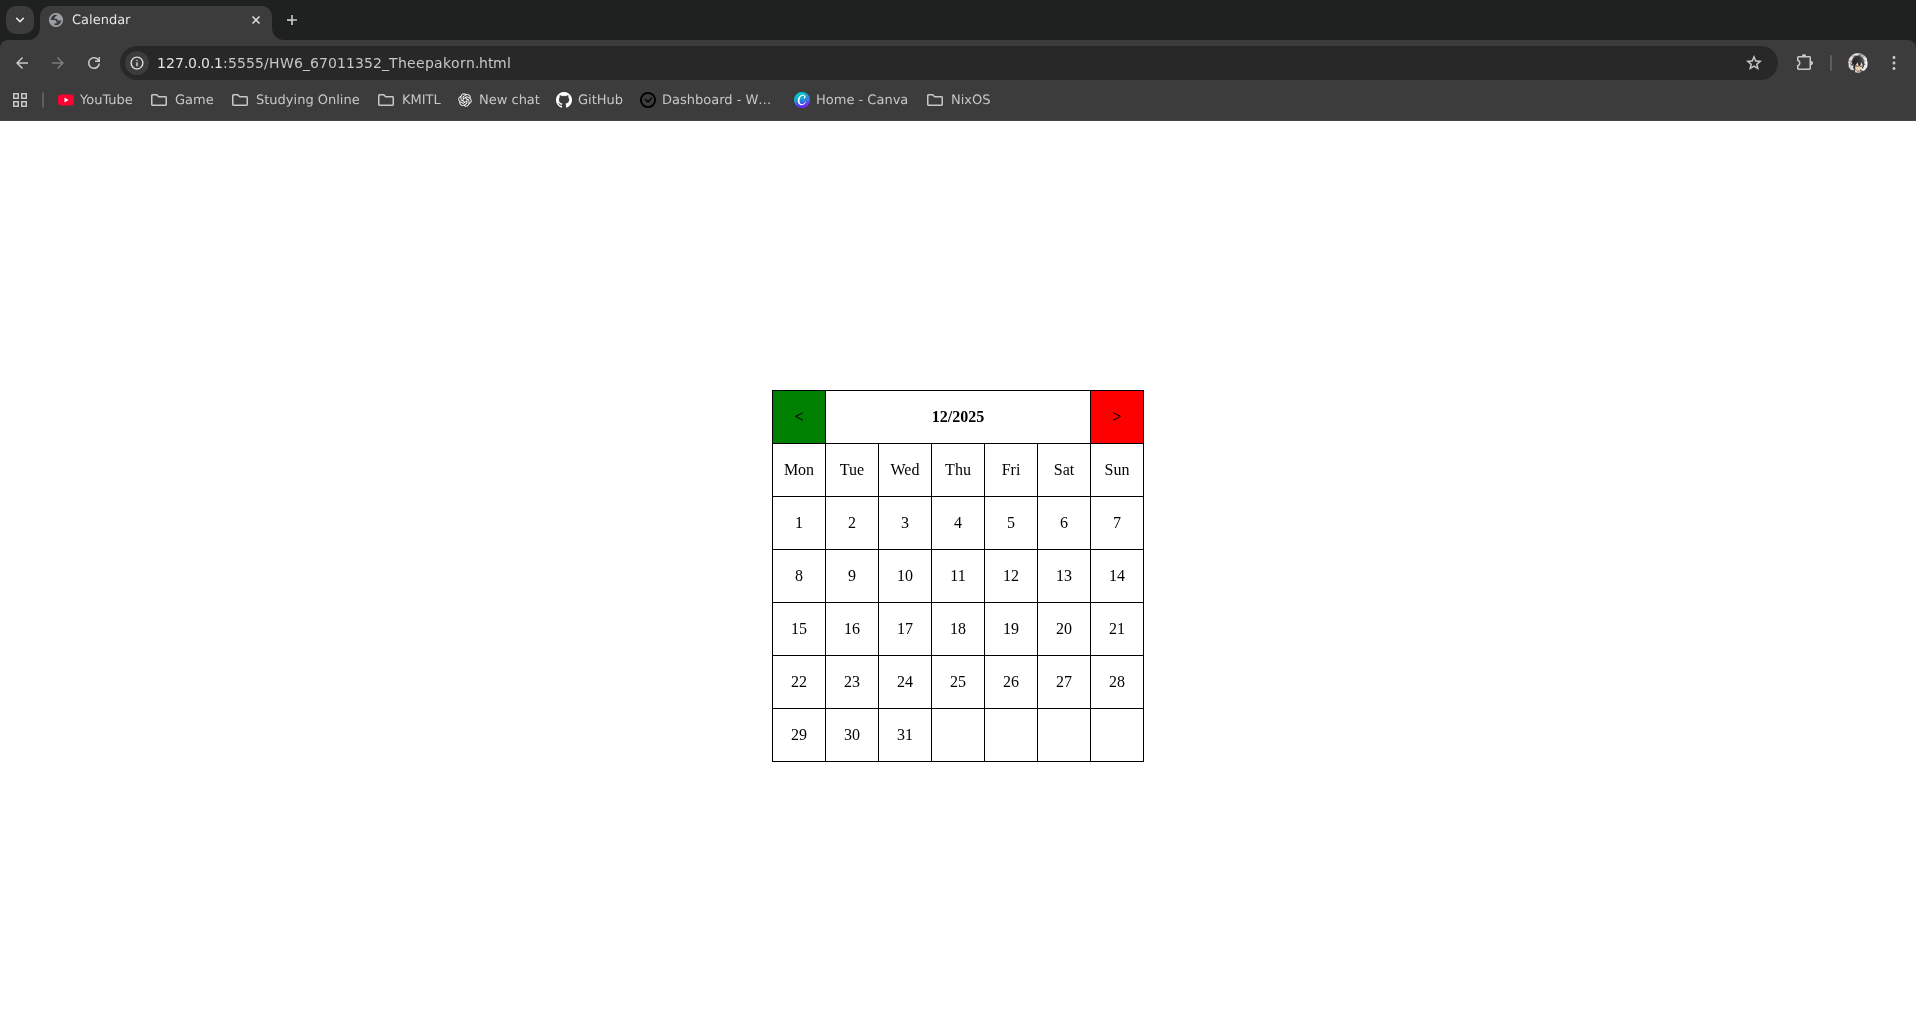
\includegraphics[width=12cm]{./images/Output12.png} \\

\end{document}
